\documentclass{standalone}
\usepackage[T1]{fontenc}
\usepackage[latin2]{inputenc}
\usepackage[english]{babel}
\usepackage{tikz}
\usepackage{times}

% Packages needed to draw 
\usetikzlibrary{calc,through,backgrounds,positioning,fit}
\usetikzlibrary{shapes,arrows,shadows} 
\usetikzlibrary{calendar}

\begin{document}
 
% Defining different types of nodes %%%%%%%%%%%%%%%%%%%%%%%%%%%%%%%%%
\tikzstyle{place}=[shape=circle, draw, minimum height=10mm]
\tikzstyle{trig}=[shape=circle, draw, dashed, minimum height=10mm]
\tikzstyle{trans}=[shape=rectangle, draw, minimum height=6mm, minimum width=12mm]
 

\centering

%OPTIONS of tikzpicture:
% scale option scales the whole picture 


%GENERAL TIPS
% cordinate system starts from left bottom corner

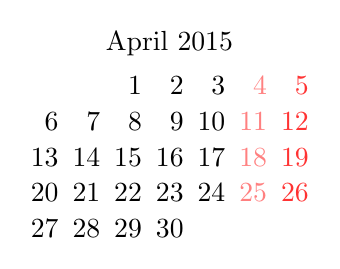
\begin{tikzpicture}[scale=1,inner sep=0.4mm]
\calendar[dates=2015-04-01 to 2015-04-30,week list, month label above centered, month text={\%mt} \%y- ]
if (Sunday) [red!80]
if (Saturday) [red!50];

\end{tikzpicture}
 
\end{document}